\documentclass[a4paper, amsfonts, amssymb, amsmath, reprint, showkeys, nofootinbib, twoside]{revtex4-2}
\usepackage{preamble}

\begin{document}

    \title{Étude du Chaos, Caractérisation des Attracteurs Chaotiques}

    \author{Antoine de Lagrave}
    \affiliation{
        Université de Sherbrooke, Département de physique, Sherbrooke, QC, Canada
    }
    \date{\today}

    \begin{abstract}
        Dans ce travail, nous étudions la caractérisation des attracteurs
        chaotiques des systèmes dynamiques. Les attracteurs chaotiques
        présentent un comportement complexe, imprévisible et non périodique,
        et constituent une caractéristique fondamentale des systèmes non
        linéaires dissipatifs. Nous utilisons diverses méthodes pour
        identifier et analyser les attracteurs chaotiques, incluant le calcul
        de(s) exposant(s) de Lyapunov. L'utilisation de méthodes numériques
        comme des algorithmes de résolution d'équations différentielles sera
        impérative et précieuse dans l'analyse numérique de tels système, de
        même que l'utilisation d'algorithme de convergence pour obtenir une
        intuition de leur comportement après un temps qui tend vers l'infini.
        Nous présentons également des exemples de ce type d'attracteurs tels
        que : l'attracteur de Lorenz, l'attracteur de Rössler, l'attracteur de
        Bouali et etc. Notre étude révèle ainsi la structure riche et complexe
        des attracteurs chaotiques et fournit des aperçus sur la dynamique
        sous-jacente des systèmes qui sont à l'origine de leur apparition.
        Dans l'ensemble, cette étude contribue à une compréhension plus
        approfondie du chaos et fournit des aperçus pour l'analyse des
        systèmes chaotiques en utilisant les attracteurs comme entité
        principale.
    \end{abstract}

    \maketitle

    \section{Introduction} \label{sec: introduction}

L'intérêt scientifique envers les systèmes chaotiques remonte au 19\up{ème}
siècle alors que Henri Poincaré étudiait le comportement des solutions du
problème à trois corps \cite{poin_carre}. Bien qu'il n'était pas évident que
ce système était de nature chaotique, la forte sensibilité aux conditions
initiales et la non périodicité des solutions étaient toutefois très présentes.
Birkhoff, Kolmogorov et Lorenz sont également d'éminents mathématiciens et
physiciens qui ont plus tard contribué considérablement dans le domaine de la
théorie du chaos respectivement grâce à la théorie ergodique, l'étude des
turbulences/algorithmes et l'étude de la météorologie. C'est d'ailleurs Edward
Lorenz qui en 1963, arrive avec l'idée \textit{l'effet papillon} selon lequel
de légères variations peuvent avoir des conséquences monstrueuses
\cite{butterfly}. Ce n'est cependant qu'au 20\up{ème} siècle que ce sujet
d'étude à connu ses plus grandes victoires et avancées. La raison principale
de cette ascension est la croissance fulgurante de l'ère numérique. L'étude de
tels systèmes est en effet particulièrement coûteuse en ce qui concerne la
partie mathématique puisqu'elle demande une grande quantité d'itérations et
c'est pourquoi les ordinateurs y sont d'une aide précieuse.

L'étude des systèmes dynamiques dissipatifs requiert régulièrement
l'intervention d'outils mathématiques et topologiques complexes pour être en
mesure d'isoler une tendance ou un comportement physique. On entend ici par
\textit{systèmes dynamiques dissipatifs} des systèmes thermodynamiques qui
agissent hors équilibre et dans lesquels les échanges d'énergie et de matière
avec l'environnement sont permis. Ces systèmes sont donc ouverts au sens
thermodynamique et sont généralement à l'origine de l'apparition d'attracteurs.
Plus précisément, les systèmes dynamiques dont la sensibilité aux conditions
initiales est élevée sont aussi appelés systèmes chaotiques. Ceux-ci sont à la
fois déterministes et imprévisibles et c'est ce mélange particulier de
simplicité et de hasard qui constitue le \textit{chaos} Il sera ici question
d'étudier les différentes propriétés et limites de certains attracteurs
fondamentaux qui émergent naturellement des systèmes dynamiques dissipatifs
tels que l'attracteur de Lorenz, Rössler et Bouali. On déterminera leur
sensibilité aux conditions initiales via l'exposant de Lyapunov et la
divergence de différente solutions grâce aux diagrammes de bifurcation. Nous
pourrons ainsi faire un lien entre ces attracteurs et de réels systèmes
physiques dans lesquels ont retrouve ces objets topologiques naturellement.


    \section{Théorie} \label{sec: theory}
    Les attracteurs sont des structures fondamentales en théorie du chaos qui jouent un rôle clé dans la compréhension du comportement chaotique des systèmes. Dans cette section, nous allons explorer en détail le concept d'attracteur en théorie du chaos, en examinant les propriétés mathématiques qui les caractérisent. 

\subsection{Attracteurs} \label{subsec: attractors}
    Pour un système dynamique dissipatif donné, l'attracteur est définit par un sous-ensemble d'états dans l'espace des phases vers lesquels la solution au système converge si les conditions initiales de ladite solution sont comprises dans le bassin d'attraction de l'attracteur. Ici, le \textit{bassin d'attraction} représente une zone de l'espace des phases dont les conditions initiales mènent à des trajectoires qui convergent vers un attracteur. Mathématiquement, on dit que le bassin d'attraction $W$ d'un attracteur $A$ est
    \begin{align}
        W(A) = \{r\in R\;\;|\;\lim_{t\to\infty} f(r, t)\in A\},
    \end{align}

    où ici $r$ représente un ensemble de condition initiales appartenant à l'espace des phases $R$ et $f(r, t)$ la trajectoire de la solution. Autrement-dit, l'attracteur est un sous-ensemble de solutions qui permet d'identifier et de prédire une tendance globale dans la trajectoire d'une solution donnée d'un système chaotique, et ce, malgré sa nature imprévisible. \\

    L'attracteur de Lorenz que l'on nommera ici $L$ est l'un des exemples les plus célèbres d'un attracteur chaotique dans la théorie des systèmes dynamiques \cite{lorenz}. Cet attracteur est le fruit d'un système dynamique non linéaire à trois dimensions qui décrit le comportement d'un fluide en mouvement. Mathématiquement, l'attracteur de Lorenz est défini par un ensemble d'équations différentielles ordinaires, qui décrivent l'évolution de trois variables dynamiques $(x, y, z)$ en fonction du temps et des paramètres $\sigma, \rho$ et $\beta$ qui régissent le comportement du système
    \begin{align}
        L = \left\{
        \begin{array}{c}
           \Dot{x} = \sigma(y - x) \\
           \Dot{y} = x(\rho - z) - y \\
           \Dot{z} = xy - \beta z, 
        \end{array}
        \right.
        \label{eq : lorenz}
    \end{align}

    où les paramètres $\sigma, \rho$ et $\beta$ sont respectivement le nombre de Prandtl, le nombre de Rayleigh et un coefficient géométrique quelconque. Un second attracteur initialement proposé par Otto Rössler en 1976 est l'attracteur de Rössler \cite{rossler}. Celui-ci possède une forme particulière et n'a qu'une seule de ses trois équations qui possède un terme non linéaire
    \begin{align}
        R = \left\{
        \begin{array}{c}
           \Dot{x} = -y - z \\
           \Dot{y} = x + ay \\
           \Dot{z} = b + z(x - c), 
        \end{array}
        \right.
        \label{eq : rossler}
    \end{align}

    avec $a, b$ et $c$ des paramètres numériques qui régissent le comportement du système. Le dernier attracteur que nous allons étudier est celui introduit par Bouali en 2013, qui est non seulement par définition très sensible aux conditions initiales, mais également à la source du phénomène unique de chevauchement d'attracteurs \cite{bouali}. Les équations différentielles non-linéaires qui décrivent cet attracteur sont
        \begin{align}
        B = \left\{
        \begin{array}{c}
           \Dot{x} = \alpha x(1 - y) - \beta z \\
           \Dot{y} = -\gamma y(1 - x^2) \\
           \Dot{z} = \mu x,
        \end{array}
        \right.
        \label{eq : bouali}
    \end{align}

    où les paramètres $\alpha, \beta, \gamma$ et $\mu$ sont une fois de plus des coefficients numériques responsables du comportement de l'attracteur.

\subsection{Exposants de Lyapunov} \label{subsec: lyapunov}
    Nous avons définit que les systèmes dynamiques dissipatifs sensibles au changement infinitésimal des conditions initiales sont chaotiques et donc que deux trajectoires peuvent se voir diverger rapidement. Soit deux positions initiales de l'espace des phases $\bm{x}(t)$ et $\bm{x}(t) + \bm{\delta}_0$ tels que montrés sur la figure \ref{fig: theo_lyapunov}
    \begin{figure}[h!]
        \centering
        \includegraphics[scale=0.3]{figs/Orbital_instability_(Lyapunov_exponent).png}
        \caption{Schéma qui exprime l'évolution de la distance entre deux trajectoires $|\bm{\delta}(t)|$ initialement espacées d'un déplacement infinitésimal $|\bm{\delta_0}|$ en fonction du temps \cite{LEs_wiki}.}
        \label{fig: theo_lyapunov}
    \end{figure}
    
    on considère qu'au temps $t=0$ ces trajectoires ont été éloignées du vecteur déplacement $\bm{\delta}_0$ tel que sa norme $|\bm{\delta}_0|$ soit infinitésimale. Dans le contexte de systèmes chaotique, on trouve qu'après un temps d'évolution $t$, la norme du déplacement entre les trajectoires est donné par
    \begin{align}
        |\bm{\delta}(t)| \simeq |\bm{\delta}_0|e^{\lambda t},
        \label{eq : lyapunov_delta}
    \end{align}

    où l'on appelle la quantité $\lambda$ \textit{l'exposant de Lyapunov}. On accède à cette quantité avec quelques manipulation
    \begin{align}
        \lambda \simeq \frac{1}{t}\ln\qty[\frac{|\bm{\delta}(t)|}{|\bm{\delta}_0|}],
    \end{align}

    où pour un système avec pas temporels discrets tels que l'itération $x_{n + 1} = f(x_n)$, se traduit par
    \begin{align}
        \lambda(x_0) = \lim_{n\to\infty}\sum_{i = 0}^{n - 1}\ln(f'(x_i)),
    \end{align}

    avec $x_0$ le point qui correspond à la condition initiale. On voit ici que pour des solutions calculées à l'aide d'algorithmes, il est possible de remplacer la limite itérative infinie par un algorithme de convergence judicieusement choisi tel que \textit{l'algorithme epsilon}. Il est cependant important de noter que jusqu'ici, nous n'avons introduit qu'un seul exposant $\lambda$ (le plus élevé conventionnellement), mais un système de dimension $N$ possède naturellement $N$ exposants de Lyapunov. On appelle ces valeurs le \textit{spectre de Lyapunov} d'un système. Ce spectre possède plusieurs propriétés intéressantes pour l'analyse des systèmes dynamiques \cite{LEs}: \\
    \begin{itemize}
        \item[$\diamond$] Les composantes du spectres sont indépendantes du métrique utilisé pour leur calcul ainsi que du choix des variables. Cela permet de conclure sur l'objectivité et la pertinence du spectre de Lyapunov. \\
        \item[$\diamond$] Si l'exposant le plus élevé du spectre est positif témoigne généralement d'instabilités exponentiellement importantes et consitue une définition de ce que l'on pourrait appeler chaos. \\
        \item[$\diamond$] La somme du spectre de Lyapunov permet de mesurer le taux contraction des volumes de l'espace des phases. Pour des systèmes dissipatifs, une somme $\sum_i\lambda_i < 0$ signifie que les volumes décroissent exponentiellement à 0 alors qu'une somme nulle implique la conservation des volumes de l'espace des phases.
    \end{itemize}

    \section{Méthode} \label{sec: method}
    L'étude et la caractérisation numérique des attracteurs chaotiques
    requiert la connaissance de plusieurs méthodes/algorithmes. L'utilisation
    du langage de \textit{haut niveau} Python est donc agréable grâce à la
    manipulation intuitive des objets mathématiques multidimensionnels et dans
    l'implémentation de diverses méthodes numériques. On explicitera ici la
    façon dont les attracteurs présentés dans la section
    \fullref{subsec: attractors} ont été simulés, comment le spectre de
    Lyapunov à été calculé et finalement l'algorithme avec lequel ce spectre a
    pu été estimé pour un temps de simulation $t\to\infty$.

\subsection{Équations différentielles} \label{subsec: res_diff}
    Les systèmes d'équations différentielles \eqref{eq : lorenz},
    \eqref{eq : rossler} et \eqref{eq : bouali} qui décrivent les attracteurs
    étudiés dans ce travail on tous pu être simulé pour des configurations
    données de l'espace des phases (ex: conditions initiales, coefficients,
    etc.). Les simulations peuvent être faites selon 4 méthodes de résolution
    soit: Euler, Prédicteur-Correcteur, Runge-Kutta (ordre 2 et 4) et
    l'utilisation de la librairie \textit{scipy} en Python \cite{SENECH}. Dans
    le cadre de ce travail, ces algorithmes possèdent tous la même forme et
    possèdent tous les mêmes paramètres obligatoires, c.-à.-d. une position
    initiale dans l'espace ($\bm{y}_0$) et une grille temporelle qui permet
    d'identifier chaque incrément de temps pour lesquels redéfinir une
    nouvelle position.

    \subsubsection{Méthode d'Euler} \label{subsubsec: euler}
    La méthode la plus simple est la méthode d'Euler. Il s'agit d'une méthode
    récursive qui manque de précision de par sa simplicité puisqu'elle ne
    permet qu'une précision à l'ordre 1 en $h$. Soit une grille temporelle
    $t_n$ dont chaque élément est espacé d'un pas $h$ et une une fonction
    vectorielle $\bm{x}(t)$, on définit la fonction $x_{n + 1}$ en utilisant
    une approximation de la dérivée
    \begin{align*}
        \bm{x}_{n + 1} \approx \bm{x}_n + h\bm{f}(\bm{x}_n, t_n),
    \end{align*}

    où $\bm{f}$ est une fonction qui évalue le système d'équations
    différentielles pour un point de l'espace-temps donné ($\bm{x}_n, t_n$).
    Cette relation permet donc à partir d'un point initial $\bm{x}_0$,
    d'obtenir la trajectoire complète.

    \subsubsection{Prédicteur-correcteur} \label{subsubsec: pred-corr}
    Une amélioration de la méthode \fullref{subsubsec: euler} est la méthode
    Prédicteur-Correcteur. Celle-ci requiert le double du nombre d'itérations
    par rapport à Euler, mais est cependant précise à l'ordre 2 en $h$. On
    procède d'abord à une prédiction sur la valeur au temps $t_{n + 1}$ de la
    fonction $\bm{x}(t)$
    \begin{align*}
        \bm{x}_{pred.} = \bm{x}_n + h\bm{f}(\bm{x}_n, t_n),
    \end{align*}
    et on corrige cette prédiction en prenant la moyenne de l'évaluation de la
    dérivée en $\bm{x}_n$ et $\bm{x}_{pred.}$, c.-à.-d.
    \begin{align*}
        \bm{x}_{n + 1} = \bm{x}_n + \frac{1}{2}h(\bm{f}(\bm{x}_n, t_n) +
        \bm{f}(\bm{x}_{pred.}, t_{n + 1})).
    \end{align*}

    \subsubsection{Runge-Kutta (ordre 2 et 4)} \label{subsubsec: runge-kutta}
    La méthode de Runge-Kutta se présente comme une forme généralisée de la
    méthode \fullref{subsubsec: pred-corr}. On procède à 2 et 4 prédictions du
    même type que Prédicteur-Correcteur pour les méthodes d'ordre 2 et 4
    respectivement. Le calcul de points médians permet de rendre la méthode de
    plus en plus précise, mais cela a effectivement un coût algorithmique
    non-négligeable ce qui fait de la méthode d'ordre 4 un bon compromis. On
    détaille cette méthode en 5 étapes
    \begin{align*}
        \bm{k}_1 &= h\bm{f}(\bm{x}_n, t_n) \\
        \bm{k}_2 &= h\bm{f}(\bm{x}_n + \bm{k}_1/2, t_n + h/2) \\
        \bm{k}_2 &= h\bm{f}(\bm{x}_n + \bm{k}_2/2, t_n + h/2) \\
        \bm{k}_4 &= h\bm{f}(\bm{x}_n + \bm{k}_3, t_n + h) \\
        \bm{x}_{n + 1} &= \bm{x}_n + \frac{1}{6}\bm{k}_1 + \frac{1}{3}\bm{k}_2
        + \frac{1}{3}\bm{k}_3 + \frac{1}{6}\bm{k}_4
    \end{align*}

    \subsubsection{Librairie \textit{scipy}} \label{subsubsec: scipy}
    On prend ici le temps de noter que pour la majorité des calculs/résultats
    qui seront présentés dans la prochaine section, la méthode de calcul la
    plus exacte et rapide s'est avérée être l'utilisation des méthodes Python
    provenant de la librairie
    \textit{scipy}\footnote{\href{https://scipy.org/}{SciPy: Fundamental
    algorithms for scientific computing in Python.}}. Ici on  réfère plus
    particulièrement aux fonctions \texttt{scipy.integrate.odeint} ainsi
    que \texttt{scipy.optimize.solve\_ivp}, deux fonctions très efficaces et
    optimisées pour résoudre des systèmes d'équations différentielles.

\subsection{Calcul du spectre de Lyapunov} \label{subsec: lyapunov_compute}
    Pour déterminer le spectre de Lyapunov dans le cas tridimensionnel
    ($\lambda_i\forall i\in\{1, 2, 3\}$), on utilisera des méthodes de calcul
    matricielles. En effet, pour déterminer comment se comporte l'espace autour
    d'un point d'une trajectoire chaotique donnée, on initialisera une matrice
    identité $U_{3x3}$. Il est possible de penser que cette matrice représente
    une sphère de rayon unitaire au temps $t=0$ de la simulation et que sa
    déformation suivant les trois directions que constituent l'espace
    tridimensionnel au cours du temps permet d'obtenir le spectre de Lyapunov.
    Pour se faire, on calcule d'abord la matrice jacobienne $J$ du système
    d'équations différentielles étudié pour chaque point de la trajectoire de
    la particule à l'intérieur de l'attracteur. Cette matrice est la matrice
    des dérivées partielles pour chaque équation du système, c.-à.-d. que pour
    un système d'équations $f$ on aurait
    \begin{align*}
        J_{ij} =
        \frac{\partial f_i}{\partial x_j}\eqtext{avec}x_j\in\{x, y, z\},
    \end{align*}
    où ici le terme $f_i$ représente l'équation différentielle $i$ du système
    et $x_j$ la variable selon laquelle dériver. Pour donner un exemple
    concret, le jacobien au point $\bm{r} = (x, y, z)$ pour l'attracteur de
    Lorenz \eqref{eq : lorenz} est la suivante:
    \begin{align*}
        J_L(\bm{r}) =
        \begin{pmatrix}
            -\sigma & \sigma & 0 \\
            \rho - z & -1 & -x \\
            y & x & -\beta
        \end{pmatrix}.
    \end{align*}

    Cette matrice $J$ joue un rôle clé dans le calcul du spectre de Lyapunov
    puisqu'elle permet d'avoir (pour tout point de la trajectoire) les taux de
    contraction/expansion de l'espace dans les directions orthogonales du
    système. En d'autres mots, ces taux de contraction/expansion donnent
    l'information sur l'évolution de trajectoires infinitésimalement voisines
    à la trajectoire originale. On reconnaît ici la définition même des
    exposants de Lyapunov donnée dans la section \fullref{subsec: lyapunov}.
    Pour continuer le calcul, on procédera, à chaque itération, à la
    multiplication de la matrice $J$ à la matrice $U$ pour obtenir la
    contraction/expansion locale à chaque point de l'espace des phases. On
    multiplie ensuite cette matrice résultante par la transposée de $U$ dans
    le but d'obtenir ces étirements dans la base de référence donnée par les
    vecteurs de $U$. Autrement dit, on obtenir les contractions/expansions à un
    instant donné via $J\cdot U$ et l'on applique celles-ci sur les vecteurs de
    la matrice $U$ pour savoir comment ses vecteurs se comportent par rapport
    au temps. À la place d'avoir seulement des taux, on obtient des mesures
    concrètes de contraction/expansion de la sphère unitaire créée au début de
    la simulation. On dira notamment que l'élément $[U^T\cdot(J\cdot U)]_{ij}$
    correspond au taux de contraction/expansion des vecteurs directeurs de la
    sphère dans la direction $i$ s'ils ont été perturbés dans la direction $j$.
    C'est d'ailleurs pour cette raison que si l'on extrait la diagonale de
    cette dernière matrice, on obtient le spectre de Lyapunov. \\

    Ainsi, en termes algorithmiques, pour chaque temps $t_i$ de la simulation,
    on procède aux étapes suivantes: \\
    \begin{itemize}
        \item[$\diamond$] Calcul de la position et de la matrice jacobienne
            $J$ associée à cette position. \\
        \item[$\diamond$] Détermine la contraction/expansion de la sphère
            initialement unitaire dans les directions $\basis{x}, \basis{y},
            \basis{z}$ grâce à $R_i = U_i^T\cdot(J_i\cdot U_i)$. \\
        \item[$\diamond$] Collecte du spectre de Lyapunov ($L_i$) en faisant
            l'extraction de la diagonale de $R_i$. \\
        \item[$\diamond$] Utilisation de transformations de Householder afin
            de rendre la matrice $R_i$ antisymétrique. \\
        \item[$\diamond$] Mise à jour des dimensions de la sphère de
            contraction/expansion grâce au produit matriciel $U_i\cdot R_i$. \\
    \end{itemize}

    En termes numériques, on arrive à procéder à toutes ces itérations en
    utilisant une fois de plus la librairie \textit{scipy}. On fabrique
    essentiellement un système d'équation matriciel que l'on intègre par
    rapport au temps via la fonction \texttt{scipy.integrate.odeint}. Le
    système injecté dans cette fonction est un système qui est une
    généralisation des étapes algorithmiques décrites un peu plus haut soit:
    \begin{align*}
        \Dot{U} = UX\betspace\Dot{L} = \diag{R}
    \end{align*}

\subsection{Algorithme de convergence} \label{subsec: convergence}
    Comme introduit dans la section \fullref{subsec: lyapunov}, puisque
    l'équation \eqref{fig: theo_lyapunov} concernant l'exposant de Lyapunov
    est une somme infinie, il est évident que ce calcul est numériquement
    impossible. Cependant, il existe une panoplie d'algorithme de convergence
    qui permettent d'estimer la valeur d'une série pour un nombre infini de
    termes en utilisant seulement quelques termes de ladite série. On utilisera
    ici l'algorithme epsilon. Une façon intuitive d'introduire l'algorithme de
    convergence epsilon est en prenant une série de valeurs quelconques
    composée de 5 termes tous identifiés par les lettres $S_{i=1, 2,\dots}$.
    On définit l'algorithme epsilon grâce à un tableau triangulaire
    \begin{figure}[h!]
        \centering
        \includegraphics[scale=0.3]{figs/epsilon_tri_array.png}
        \caption{Tableau triangulaire représentant le mode de fonctionnement
        de l'algorithme epsilon pour une série de 5 termes \cite{SENECH}.}
        \label{fig: epsilon_tri_array}
    \end{figure}
    Soit la figure \ref{fig: epsilon_tri_array}, on voit que chaque élément du
    tableau est déterminé grâce aux trois éléments qui figurent en haut à
    gauche, directement à gauche et en bas à gauche jusqu'à arriver au dernier
    élément puisque cela forme un triangle. Numériquement, on initialise
    d'abord la première colonne de valeur comme
    \begin{align*}
        \epsilon_{k=-1}^{(n)} = 0\betspace\epsilon_{k=0}^{(n)} = S_n,
    \end{align*}
    pour ensuite déterminer les autres termes du tableau grâce à l'expression
    \begin{align*}
        \epsilon_{k + 1}^{(n)} = \epsilon_{k - 1}^{(n + 1)} +
        \frac{1}{\epsilon_{k}^{(n + 1)} + \epsilon_{k}^{(n)}}\eqtext{}\forall
        n, k\in\mathbb{N}
    \end{align*}
    où l'on considère qu'il y à $n$ lignes et $k$ colonnes dans le tableau
    triangulaire. On note également que les termes dans les colonnes d'indices
    impairs ne constituent pas de bonnes approximations pour la série $S_n$ et
    donc si l'on donne à l'algorithme une nombre de termes impairs, il est
    impératif d'ajouter une colonne nulle à l'indice $k=-1$ de sorte à ce qu'à
    la fin de l'algorithme la valeur retournée soit précisément celle qui soit
    le pic du triangle.


    \section{Résultats} \label{sec: resultats}

\subsection{Trajectoires} \label{subsec: res_trajectories}
    Soit les figures \ref{fig: traj_lorenz}, \ref{fig: traj_rossler} et \ref{fig: traj_bouali} qui présentent les résultats pour la simulation des attracteurs (Lorenz, Rössler et Bouali) définis mathématiquement dans la section \fullref{sec: theory}. On voit sur lesdites figures la trajectoires d'une particule de masse unité dans les systèmes dynamiques dissipatifs représentés par les différents attracteurs. Étonnement, les trajectoires montrées sur ces figures ne semble pas du tout chaotiques, et se rapprochent d'arrangements très bien organisés voir même prédictibles. Une fois de plus, la subtilité réside dans la sensibilité de ces systèmes aux conditions initiales. Il est d'ailleurs à noter que ces figures sont des trajectoires qui proviennent d'\textbf{une seule} position initiale à chaque fois. Pour voir à quel point ces attracteurs sont chaotiques ou non, nous devrions exécuter la simulation pour une multitude de coordonnées initiales et ainsi observer la divergence très précoce entre les solutions. Un bon indicateur de signature chaotique est le spectre de Lyapunov et c'est pourquoi nous allons analyser ce spectre en utilisant les mêmes trajectoires attractives. \\

    Il est également intéressant d'observer sur les figures \ref{fig: traj_lorenz}, \ref{fig: traj_rossler} et \ref{fig: traj_bouali} que le théorème d'unicité des solutions d'équations différentielles ordinaires est vérifié \cite{uniqueness}. On observe effectivement aucun croisement dans les trajectoires obtenues.

\subsection{Spectre de Lyapunov} \label{subsec: res_lyapunov}
    Considérons les figures \ref{fig : lyaps_lorenz}, \ref{fig : lyaps_rossler} et \ref{fig : lyaps_bouali}, sur lesquelles ont observe le calcul du spectre de Lyapunov en fonction du temps pour les trajectoires attractives discutées dans la section \fullref{subsec: res_trajectories}. Il est intéressant d'observer la précieuse utilisation de l'algorithme de convergence epsilon introduit dans la section \fullref{subsec: convergence}. La convergence est pertinente et permet bien d'identifier le comportement à long terme ($\lim_{t\to\infty}\lambda_i(t)$) du spectre de Lyapunov pour la trajectoire des attracteurs étudiés. \\

    On remarque premièrement, pour tous les attracteurs, que l'exposant de Lyapunov maximal $\lambda_1$ est positif. Comme introduit dans la section \fullref{subsec: lyapunov}, il s'agit-là d'une signature typique de chaos. Mathématiquement, cela signifie que dans la direction associée à l'exposant $\lambda_1$ deux trajectoires voisines divergent exponentiellement rapidement dans le temps et donc que de toutes petites perturbations peuvent mener à des trajectoires très différentes. On peut ici faire un lien avec la contraction/expansion de l'espace des phases modélisée par l'évolution du volume de la sphère unitaire $U$ vis-à-vis du signe obtenu pour les composantes du spectre de Lyapunov. \\

    Ensuite, on remarque que dans les résultats obtenus, deux des trois exposants sont négatifs. Cela signifie logiquement que deux trajectoires voisines tendent à converger au sein de l'attracteur et demeurer près l'une de l'autre. Physiquement, on peut aussi dire que des exposants négatifs indiquent que les systèmes étudiés sont dissipatifs (perdent de l'énergie au cours du temps) et donc qu'il est normal d'observer la convergence de certaines trajectoires comme par exemple lorsque l'on étudie un oscillateur harmonique amorti. \\

    Finalement, on voit que certains des exposants de Lyapunov sont nuls. Ces derniers n'impliquent pas de comportement chaotique particuliers. On peut conclure que mathématiquement, une perturbation d'une trajectoire ayant un exposant de Lyapunov nul peut se voir diverger mais seulement de façon logarithmique. On appelle ce phénomène: \textit{comportement quasi-périodique}.

\onecolumngrid
\vspace{2cm}

    \begin{figure}[h!]
        \centering
        \includegraphics[scale=0.6]{figs/trajectories/traj_lorenz.png}
        \caption{Trajectoire obtenue pour la simulation d'une particule de masse unité dans le bassin d'attraction de l'attracteur de Lorenz ayant comme position initiale $\bm{r}_0 = (1, 0, -1)$ ainsi que pour un temps de 100 secondes avec un pas de $h = 0.01$.}
        \label{fig: traj_lorenz}
    \end{figure}
    \vspace{1cm}
    \begin{figure}[h!]
        \centering
        \includegraphics[scale=0.6]{figs/trajectories/traj_rossler.png}
        \caption{Trajectoire obtenue pour la simulation d'une particule de masse unité dans le bassin d'attraction de l'attracteur de Rössler ayant comme position initiale $\bm{r}_0 = (1, 1, -1)$ ainsi que pour un temps de 1000 secondes avec un pas de $h = 0.001$.}
        \label{fig: traj_rossler}
    \end{figure}

\clearpage
    
    \begin{figure}[h!]
        \centering
        \includegraphics[scale=0.5]{figs/trajectories/traj_bouali.png}
        \caption{Trajectoire obtenue pour la simulation d'une particule de masse unité dans le bassin d'attraction de l'attracteur de Bouali ayant comme position initiale $\bm{r}_0 = (0.2, 0.2, -0.08)$ ainsi que pour un temps de 1000 secondes avec un pas de $h = 0.001$.}
        \label{fig: traj_bouali}
    \end{figure}

    \begin{figure}[h!]
        \centering
        \begin{minipage}{0.49\textwidth}
          \centering
          \includegraphics[scale = 0.4]{figs/lyapunovs/lyap_lorenz.png}
          \subcaption{}
          \label{fig: lyap_lorenz}
        \end{minipage}
        \begin{minipage}{0.49\textwidth}
          \centering
          \includegraphics[scale = 0.4]{figs/lyapunovs/lyap_lorenz_zoom.png}
          \subcaption{}
          \label{fig: lyap_lorenz_zoom}
        \end{minipage}
        \caption{Spectre de Lyapunov ($\lambda_i\forall i\in\{1, 2, 3\}$) dans la simulation de l'attracteur de Lorenz. (a) Spectre complet. (b) Mise en évidence du comportement pour les exposants $\lambda_1$ et $\lambda_2$ étant donnée la superposition et le bruit.}
        \label{fig : lyaps_lorenz}
    \end{figure}

    \begin{figure}[h!]
        \centering
        \begin{minipage}{0.49\textwidth}
          \centering
          \includegraphics[scale = 0.4]{figs/lyapunovs/lyap_rossler.png}
          \subcaption{}
          \label{fig: lyap_rossler}
        \end{minipage}
        \begin{minipage}{0.49\textwidth}
          \centering
          \includegraphics[scale = 0.4]{figs/lyapunovs/lyap_rossler_zoom.png}
          \subcaption{}
          \label{fig: lyap_rossler_zoom}
        \end{minipage}
        \caption{Spectre de Lyapunov ($\lambda_i\forall i\in\{1, 2, 3\}$) dans la simulation de l'attracteur de Rössler. (a) Spectre complet. (b) Mise en évidence du comportement pour les exposants $\lambda_1$ et $\lambda_2$ étant donnée la superposition et le bruit.}
        \label{fig : lyaps_rossler}
    \end{figure}

    \clearpage

    \begin{figure}[h!]
        \centering
        \begin{minipage}{0.49\textwidth}
          \centering
          \includegraphics[scale = 0.4]{figs/lyapunovs/lyap_bouali.png}
          \subcaption{}
          \label{fig: lyap_bouali}
        \end{minipage}
        \begin{minipage}{0.49\textwidth}
          \centering
          \includegraphics[scale = 0.4]{figs/lyapunovs/lyap_bouali_zoom.png}
          \subcaption{}
          \label{fig: lyap_bouali_zoom}
        \end{minipage}
        \caption{Spectre de Lyapunov ($\lambda_i\forall i\in\{1, 2, 3\}$) dans la simulation de l'attracteur de Bouali. (a) Spectre complet. (b) Mise en évidence du comportement pour les exposants $\lambda_1$, $\lambda_2$ et $\lambda_3$ étant donnée la superposition et le bruit.}
        \label{fig : lyaps_bouali}
    \end{figure}

\twocolumngrid


    \section{Conclusion} \label{sec: conclusion}
    Pour conclure, cette étude théorique et numérique de surface au sujet des attracteurs chaotiques a permis de comprendre comment caractériser ces entités topologiques grâce à certaines méthodes numériques et au calcul d'indicateurs comme le spectre de Lyapunov. D'abord en dressant un portrait théorique puis en développant des méthodes numériques telles que la résolution d'équations différentielles, la décomposition de matrices $QR$ ainsi que la convergence de séries à l'aide du langage Python. \\

    Ce processus à permis de vérifier le théorème d'unicité concernant les trajectoires obtenues numériquement. Trajectoires qui constituent les solutions aux systèmes d'équations différentielles qui définissent les attracteurs étudiés. Il a également été possible de conclure sur le comportement des attracteurs par rapport au signe des éléments de leur spectre de Lyapunov par rapport au temps. On a pu observer que les attracteurs chaotiques étudiés avaient bel et bien une signature chaotique au sens de ce spectre ($\lambda_1 > 0$) notamment grâce à la convergence des valeurs des composantes du spectre grâce à l'approximation donnée par l'algorithme epsilon. \\

    Pour poursuivre ce projet, il serait intéressant de prendre d'autres indicateurs tels que les diagrammes de bifurcations de certains systèmes dynamiques afin de voir où apparaissent mathématiquement ces attracteurs dans l'évolution d'un système \cite{bifurcation}. On aurait également pu analyser les points critiques des différents attracteurs.

    \appendix
    \section{Algorithme epsilon} \label{sec: annexe_epsilon}
    Soit la série de Gregory pour la fonction $\arctan(x)$
    \begin{align*}
        \arctan(x) = \sum_{n = 0}^\infty(-1)^n\frac{x^{2n + 1}}{2n + 1}
        = x - \frac{x^3}{3} + \frac{x^5}{5} - \frac{x^7}{7} + \dots,
        \label{eq: gregory}
    \end{align*}

    connue pour sa lente convergence. Si l'on pose $x = 1$ dans cette série,
    nous aurions d'un côté $\arctan(1) = \pi$ et de l'autre un série qui
    converge lentement vers cette même valeur. On peut donc se servir, pour
    accélérer la convergence de l'algorithme epsilon définit sur la figure
    \ref{fig: epsilon_tri_array} pour vérifier notre implémentation. Voici un
    graphique qui montre l'erreur commise sur la valeur de $\pi$ de la
    librairie \texttt{numpy} en fonction du nombre de terme dans la série de
    Gregory
    \begin{figure}[h!]
        \centering
        \includegraphics[scale=0.4]{figs/error_percentage.png}
        \caption{Erreur sur l'extrapolation de la série de Gregory (en prenant
        les 12 premiers termes) via l'algorithme epsilon.}
        \label{fig: epsilon_error}
    \end{figure}
    On voit ici sur la figure \ref{fig: epsilon_error} que l'algorithme fait
    effectivement converger la série vers la valeur attendue. On remarque
    qu'avec seulement 5 termes dans la série de Gregory, on peut avoir de très
    bonnes estimations
    \begin{align*}
        \frac{\text{estimation}}{\text{np.pi}}\cdot 100 \simeq
        \frac{3.142342342342342}{3.141592653589793}\cdot 100 \simeq  0.024\%
    \end{align*}

    \section{Théorème d'unicité} \label{sec: annexe_uniqueness}
    \begin{figure}[h!]
        \centering
        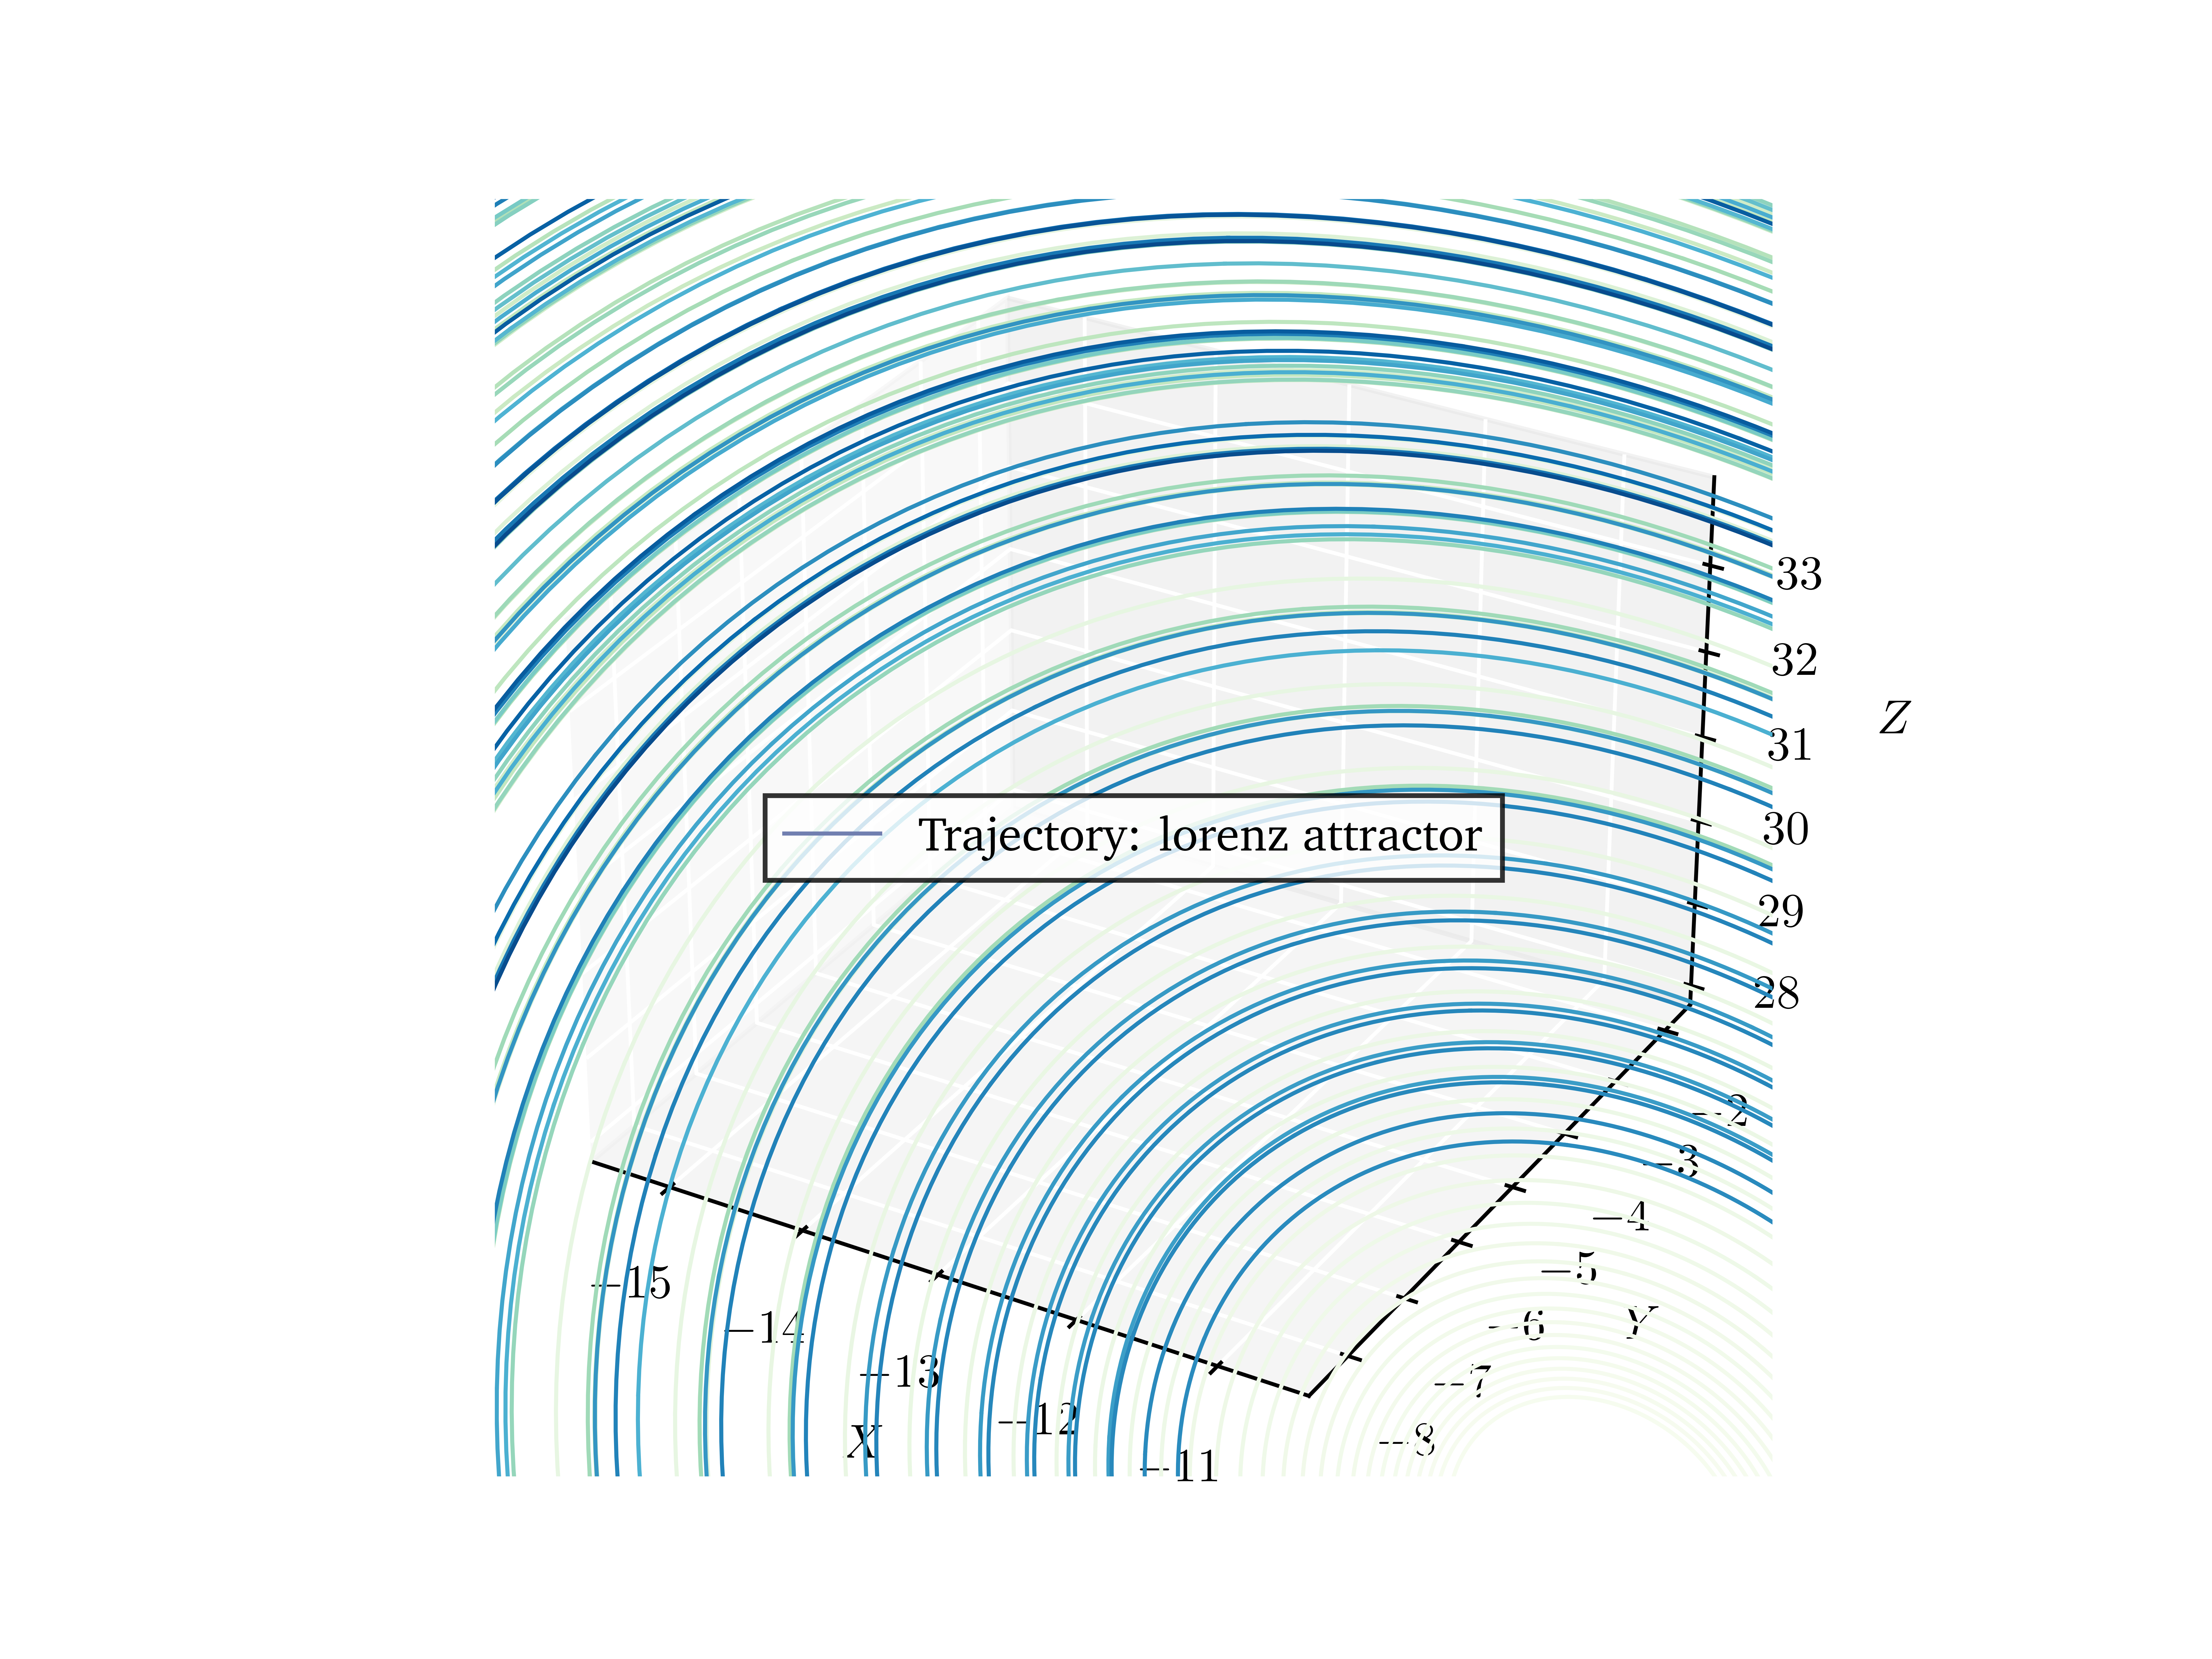
\includegraphics[scale=0.4]{figs/trajectories/unicity_lorenz.png}
        \caption{Démonstration qualitative du théorème d'unicité des solutions
        d'équations différentielles ordinaires du premier ordre à l'aide d'une
    trajectoire de l'attracteur de Lorenz.}
        \label{fig: lorenz_uniqueness}
    \end{figure}


    \bibliography{refs}

\end{document}
